\chapter{Apresentação e Análise dos Resultados}
O objeto deste trabalho é um sistema que faz o gerenciamento e a escalação automática de militares. O presente capítulo busca apresentar as funcionalidades implementadas no sistema e os passos necessários para realizar o build da aplicação.

\section{Sistema}

O sistema foi desevolvido utilizando o método de containerização, ou seja cada serviço tem o seu container. Para se construir a aplicação é necessário clonar o repositório, disponível \url{https://github.com/daniboyBr/tcc-escala-permanencia-v2}, e seguir os passos descritos no arquivo README.md. Após seguir todos os passos o sistema pode ser acesso em \url{http://localhost:8080}. Para se testar a aplicação, a base de dados foi populada com dados fictícios, podendo o perfil de administrador ser acessado com o e-mail "admin@permanencia.com" e a senha "123456789".

\subsection{Acessando o sistema}

A página inicial do sistema exibe o formulário de login, apresentada na \ref{fig:login}, é por meio dele que todo militar terá acessso as funcionalidades, sendo que algumas delas só é acessível para o usuário administrador do sistema.

\begin{figure}[!htb]
    \centering
    \caption{Tela de Login}
    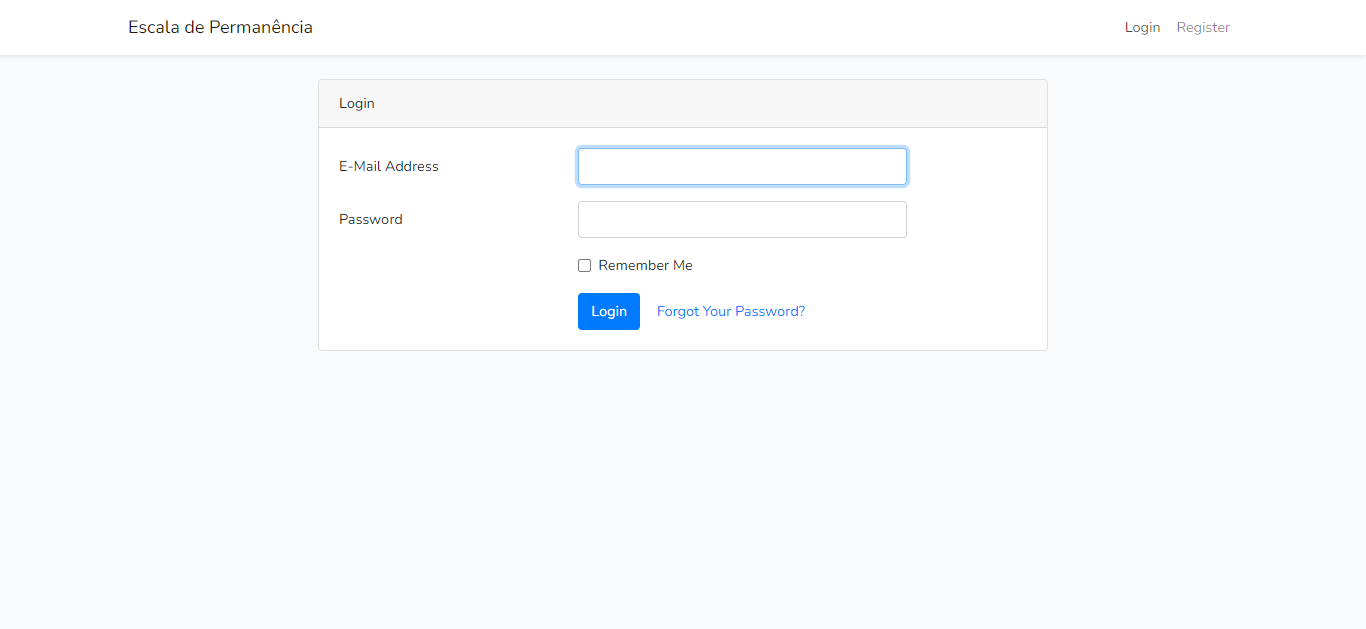
\includegraphics[width=0.8\textwidth]{images/1 - Pagina Inicial - Tela de Login.png}
    \label{fig:login}
\end{figure}

\subsection{Registrando-se no Sistema}

Na Figura \ref{fig:singnup} é mostrada a tela em que o militar deve realizar o seu cadastro, sendo que os campos e-mail e identidade devem ser únicos para cada militar.

\begin{figure}[!htb]
    \centering
    \caption{Tela de Cadastro de Militar}
    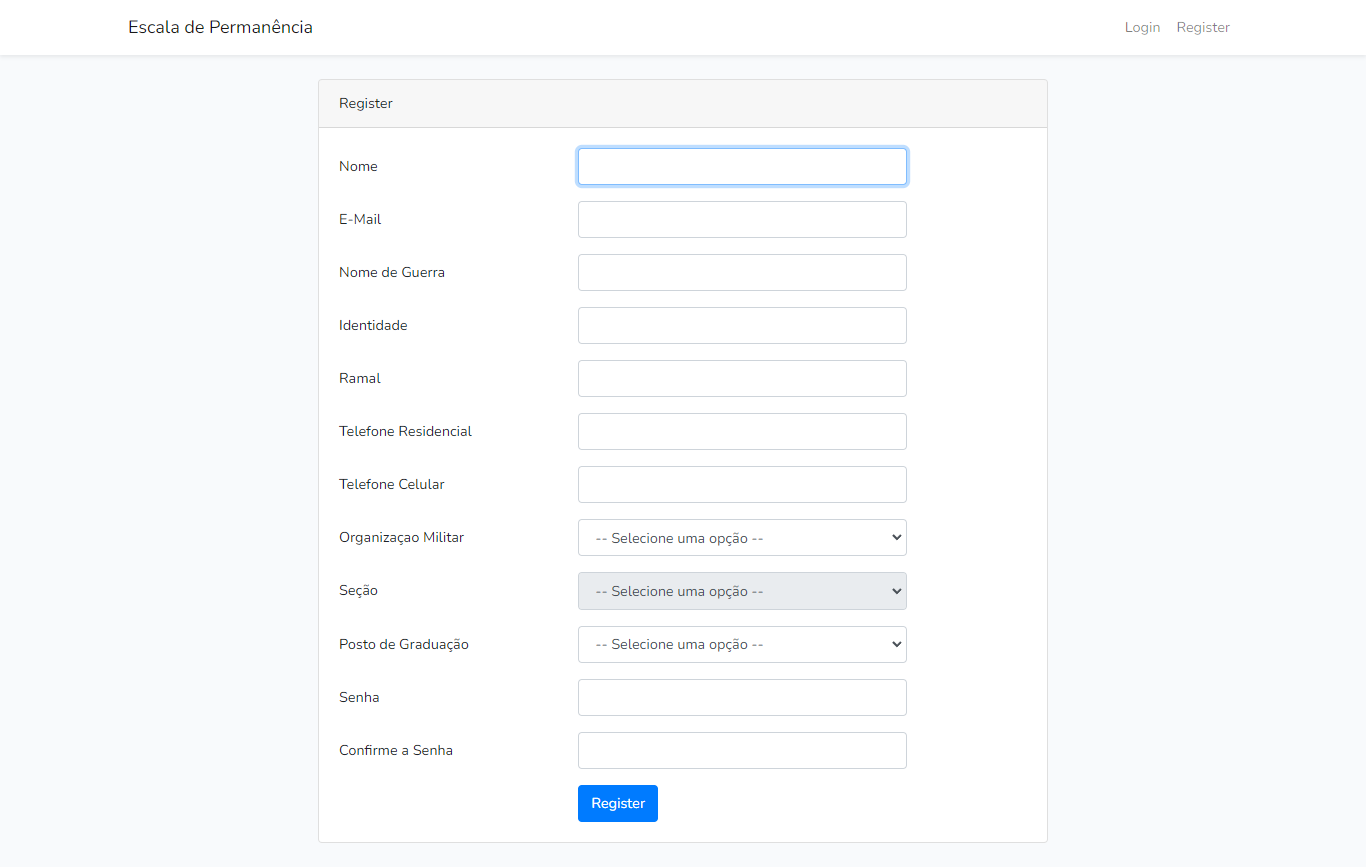
\includegraphics[width=0.8\textwidth]{images/2 - Tela de Cadastro.png}
    \label{fig:singnup}
\end{figure}

O militar, após ter efetuado cadastro, consegue ter acesso ao sistema, porém seu cadatro permanece inativo até que um usuário com perfil de administrador ativar seu cadastro, conforme apresentado na Figura \ref{fig:userinative}

\begin{figure}[!htb]
    \centering
    \caption{Tela de Militar Inativo}
    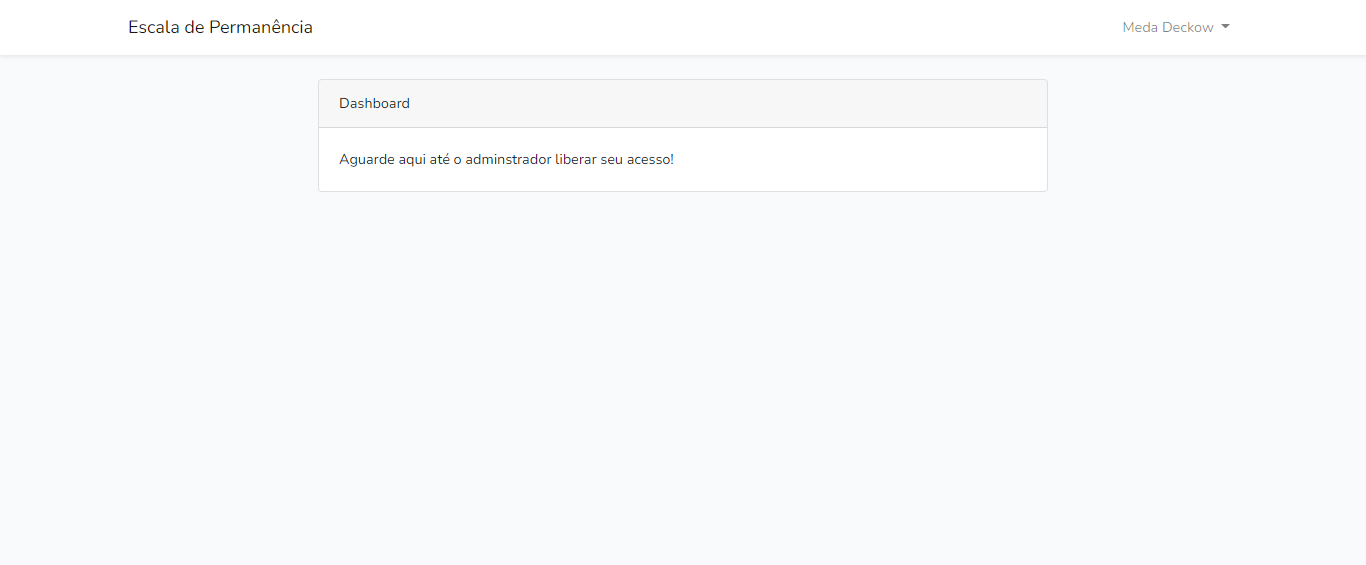
\includegraphics[width=0.8\textwidth]{images/3 - Tela de Militar Inativo.png}
    \label{fig:userinative}
\end{figure}

\subsection{Escala de Serviço}

Ao ter acesso ao sistema, com o cadastro ativo, o militar consegue visualizar a escala do dia corrente, tendo a possibilidade de pesquisar a escalação em datas futuras ou passadas por meio do filtro de data, conforme, apresentado na Figura \ref{fig:escalaservico}.

\begin{figure}[!htb]
    \centering
    \caption{Tela da Escala de Serviço}
    \includegraphics[width=0.8\textwidth]{images/4 - Tela de Visualizacao da Escala de Serviço.png}
    \label{fig:escalaservico}
\end{figure}

Na Figura \ref{fig:escalaservico}, é mostrado o botão livro, é através desse botão que o militar, no dia da sua escalação ao acessar o sistema, consegue relatar toda e qualquer ocorrência após o término do serviço, esse relato pode ser preechido no formulário apresentado na Figura \ref{fig:livroregistro}, uma vez registrado não se pode mais alterar a ocorrência informada.

\begin{figure}[!htb]
    \centering
    \caption{Tela Livro de Registro}
    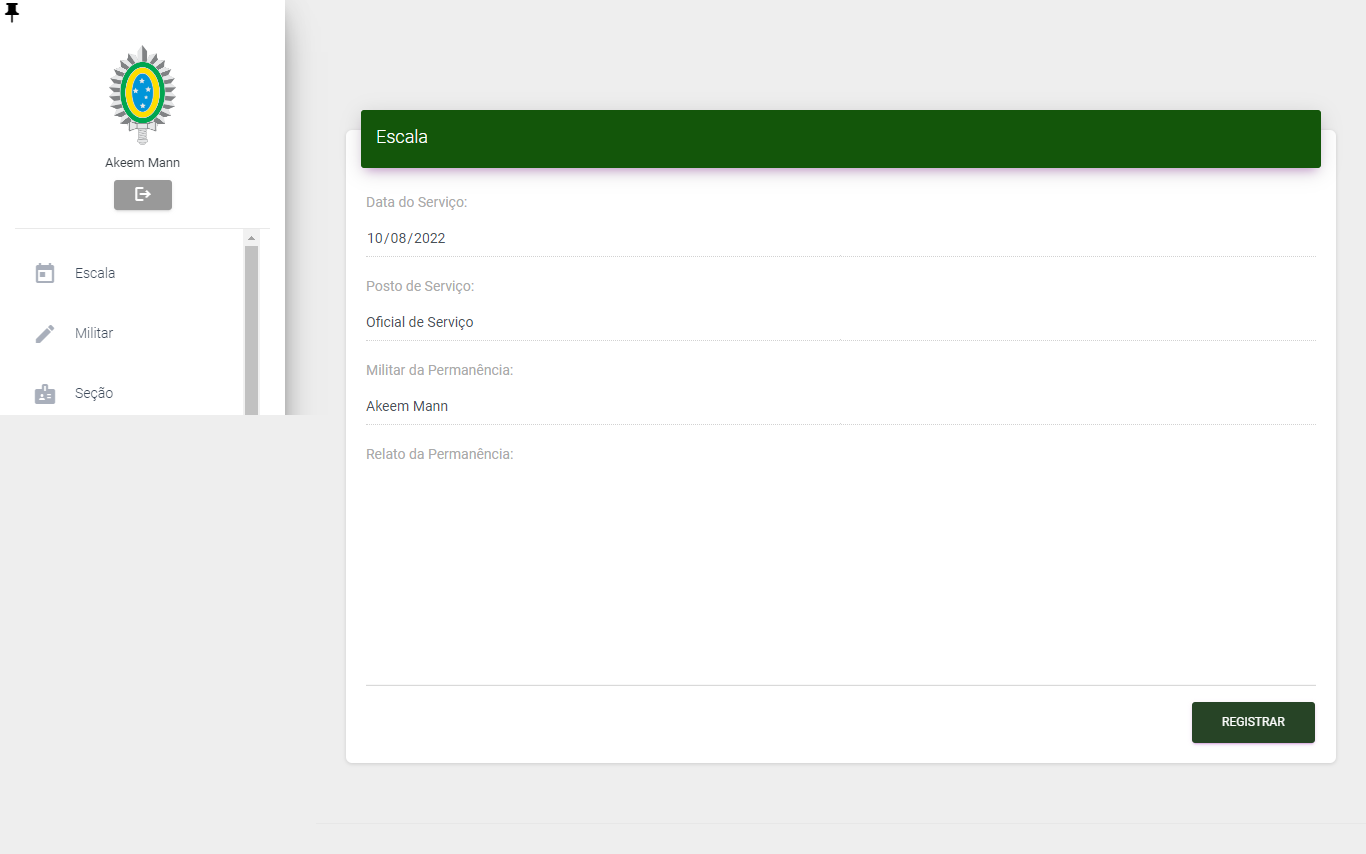
\includegraphics[width=0.8\textwidth]{images/5 - Tela Livo de Registro.png}
    \label{fig:livroregistro}
\end{figure}


\subsection{Escalação Automática de Militares}

A geração da escala acontece por debaixo dos panos. O Laravel disponibiliza uma classe chamada Command, a qual é necessário extender para criar um comando personalizado. Ao extender essa classe, foi implementadao o método handle, responsável por conter toda lógica para escalar e regras para escalar os militares,  conforme apresentado no Algorítimo \ref{lst:algofirst}.

\begin{center}
\noindent\begin{minipage}[t]{0.80\linewidth}
\begin{lstlisting}[frame=single, caption={Classe responsável por gerar escala}, label={lst:algofirst}]
class DailyScale extends Command
{
    protected $signature = 'scale:daily';
    /**  ommited code  */
    public function handle()
    {
        /**  logic to generate scale  */
    }
}
\end{lstlisting}
\end{minipage}
\end{center}

Ao se criar um comando personalizado no laravel, o mesmo ainda não é disparado de imediato, foi necessário configurá-lo na classe Kernel que extende de ConsoleKernel, para isso obrigatoriamente devemos informar um comando e a frequência na função schedule, conforme mostrado no Algorítmo \ref{lst:algosecond}. A escalação automática foi está para rodar todo dia a meia-noite.

\begin{center}
\noindent\begin{minipage}[t]{0.80\linewidth}
\begin{lstlisting}[frame=single, caption={Configuração da geração da escala}, label={lst:algosecond}]
class Kernel extends ConsoleKernel
{
    protected $commands = [
        DailyScale::class
    ];
    protected function schedule(Schedule $schedule)
    {
        $schedule->command('scale:daily')->daily();
    }
    /**  ommited code  */
}
\end{lstlisting}
\end{minipage}
\end{center}

\subsection{Notificação de Militares}

Quando a escala é gerada, um e-mail é enviado para o militar, no e-mail que ele cadastrou no sistema, conforme a Figura \ref{fig:notification}. Esse mesmo e-mail possui um link de confirmação, que ao ser clicado confirma que o militar esta ciente de sua escalação.

\begin{figure}[H]
    \centering
    \caption{Notificação do Militar}
    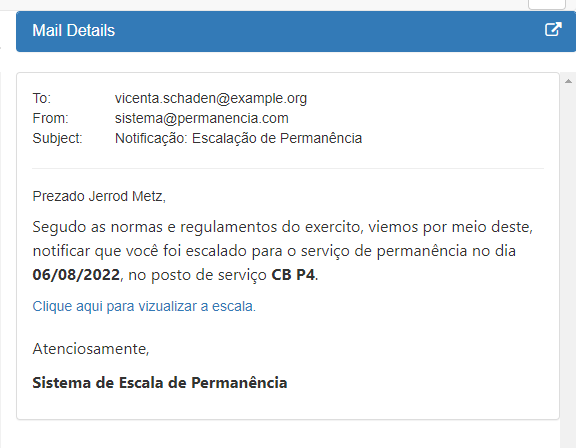
\includegraphics[width=0.8\textwidth]{images/6 - Email enviado.png}
    \label{fig:notification}
\end{figure}

Na Figura \ref{fig:notificationreplace}, mostra o e-mail enviado ao militar caso haja alguma alteração na escala, o mesmo também deve confirmar que está ciente de que houve uma troca na escala e ambos os militares são notificados, o que estava escala antes da troca e o militar que vai realizar a troca.

\begin{figure}[H]
    \centering
    \caption{Notificação de Troca de Militar}
    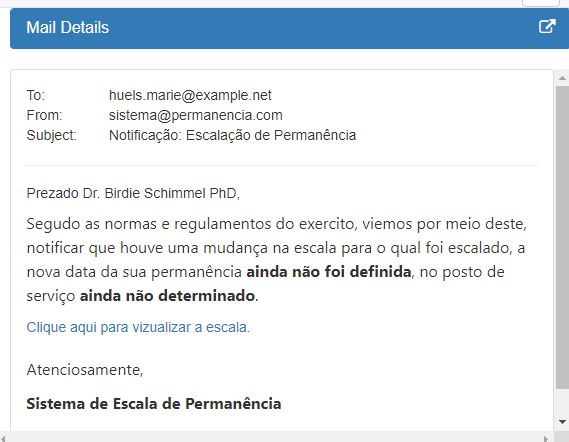
\includegraphics[width=0.8\textwidth]{images/6 - Email enviado Troca.png}
    \label{fig:notificationreplace}
\end{figure}

\subsection{Troca de Militares}

O usuário adminstrador ou escalante, só pode executar uma ação na escala, que é a troca de militares. A troca de militaress só é possível se a escala não estiver fechada, ou seja, se a escala não for da data corrente ou se já passou da data do serviço. Quando a troca de militar está habilitada aparece o botão trocar, conforme apresentado na  Figura \ref{fig:replace}.

\begin{figure}[!htb]
    \centering
    \caption{Troca de Militar}
    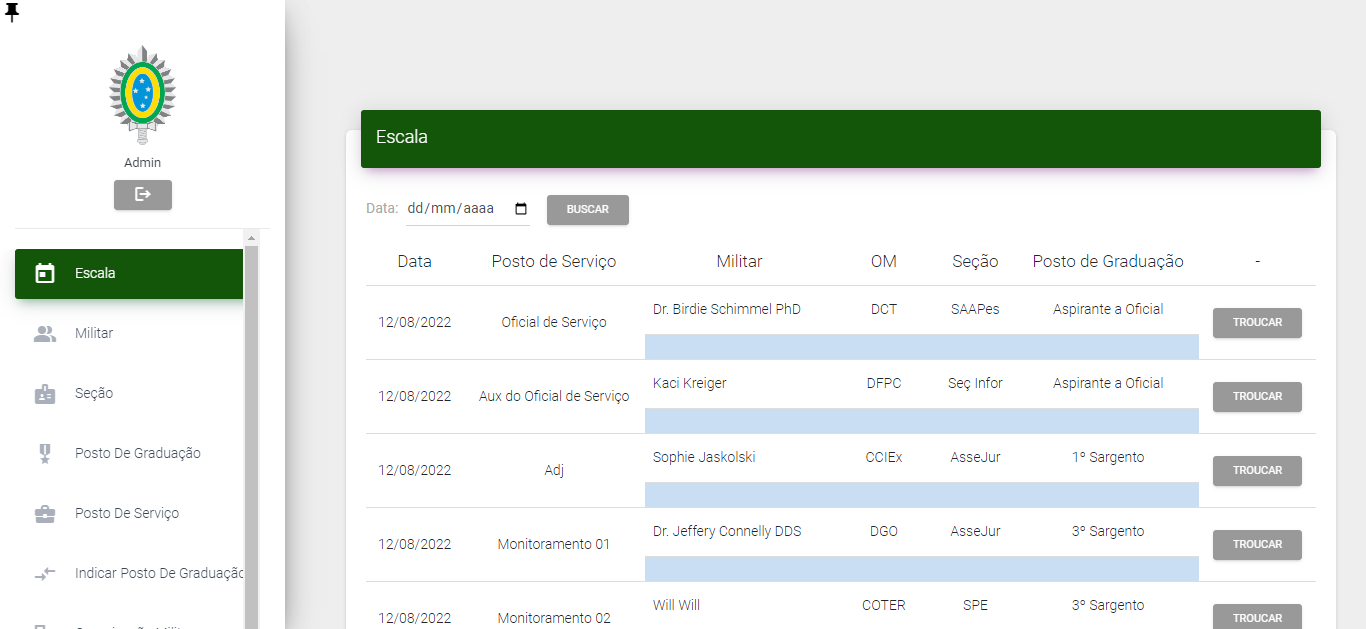
\includegraphics[width=0.8\textwidth]{images/7 - Troca de Militar.png}
    \label{fig:replace}
\end{figure}

Quando clicado no botão de troca o administrador é redirecionado pra uma página que contém o formúlario para efetuar a troca. Primeiro é  necessário buscar o militar que vai substituir o militar escalado, para isso é preciso informar a identidade do militar, conforme a Figura \ref{fig:formreplace}.

\begin{figure}[!htb]
    \centering
    \caption{Formulário para Troca de Militar}
    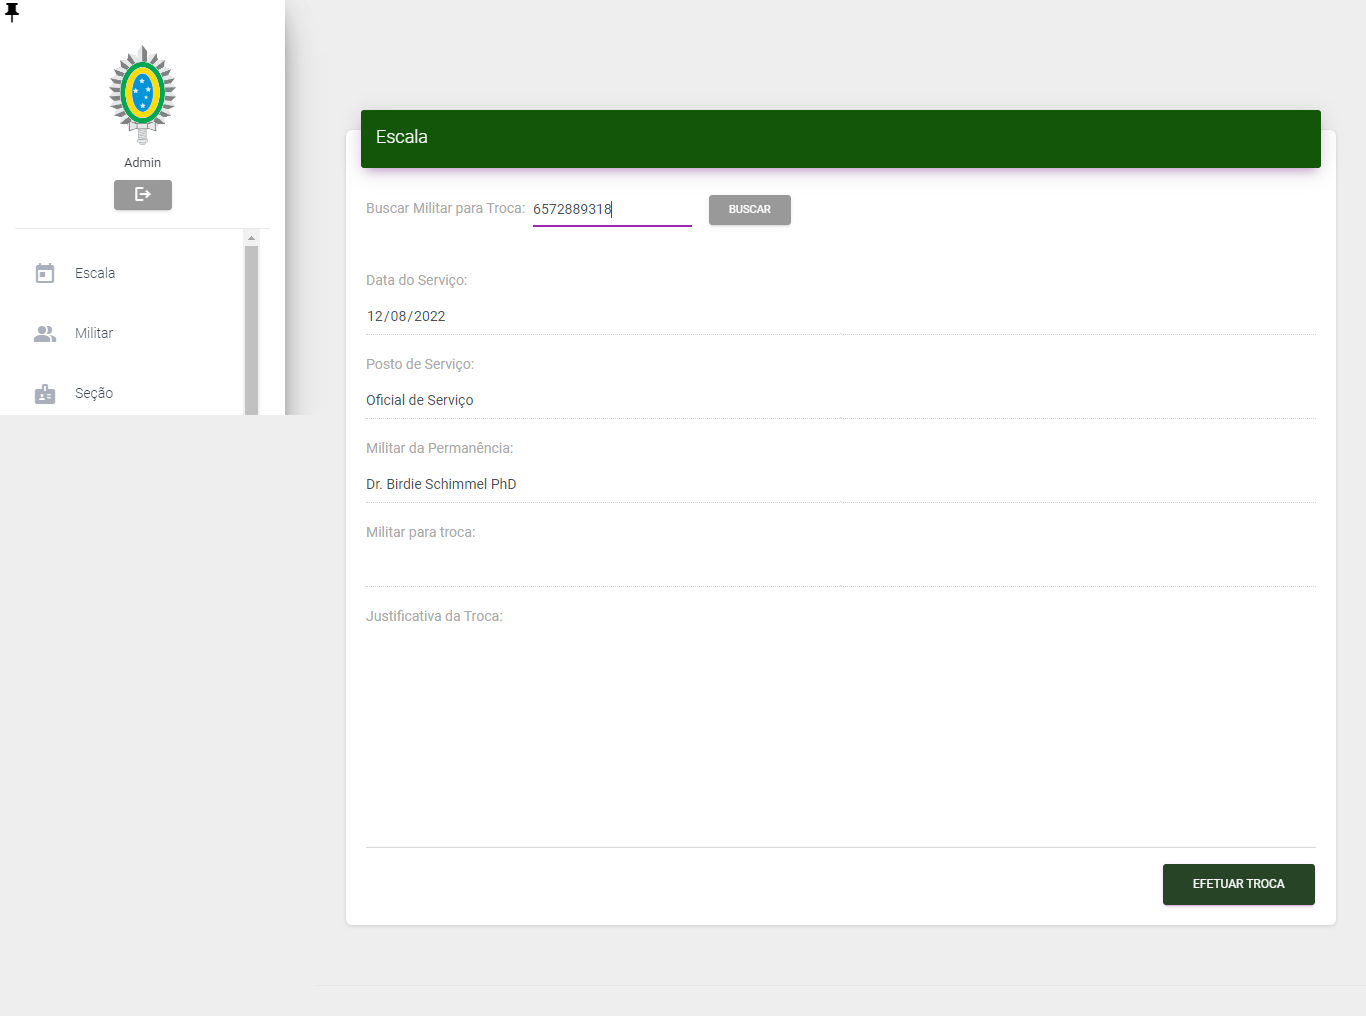
\includegraphics[width=0.8\textwidth]{images/7 - Troca de Militar - 2.png}
    \label{fig:formreplace}
\end{figure}

Para efetivar a troca, o militar que irá substituir o militar escalado deve possuir a mesma grauação configurarada para aquele serviço, senão será apresentada a mensagem demonstrada na Figura \ref{fig:formreplaceerror}.

\begin{figure}[!htb]
    \centering
    \caption{Erro de Gradução Necessária}
    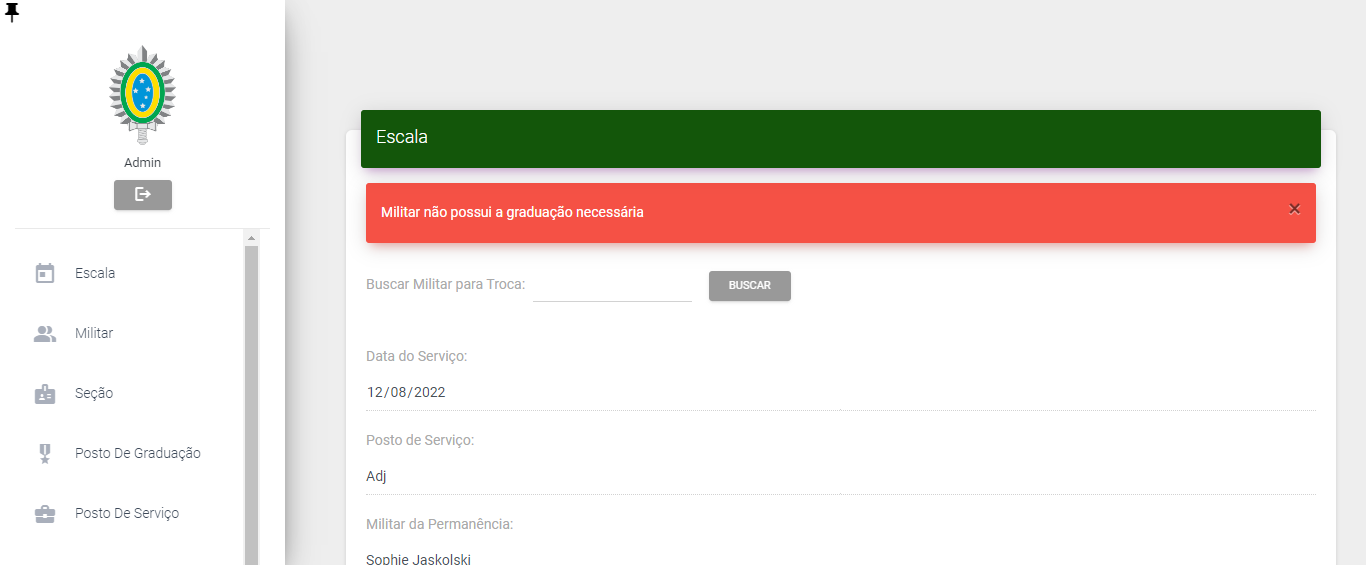
\includegraphics[width=0.8\textwidth]{images/7 - Erro Troca de Militar - Graduação.png}
    \label{fig:formreplaceerror}
\end{figure}

A Figura \ref{fig:formreplaceerror2} também demonstra um outro erro que pode ocorrer caso o administrador tente cadastrar um militar que estaja impedido naquela data.

\begin{figure}[!htb]
    \centering
    \caption{Erro de Militar Impedido}
    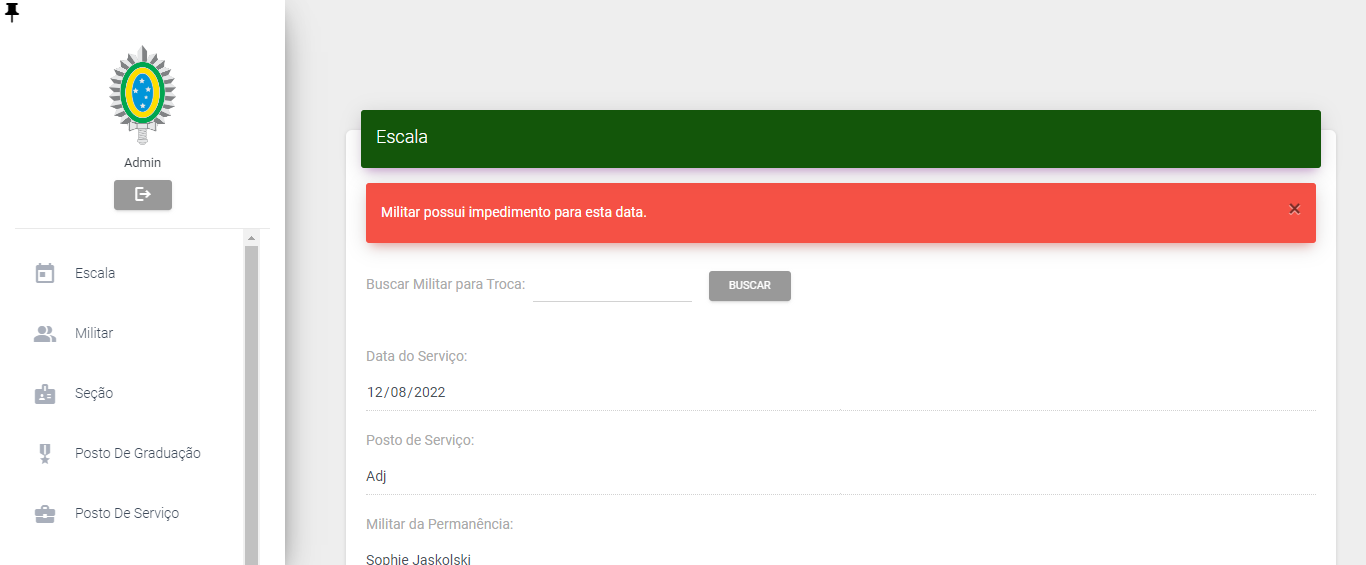
\includegraphics[width=0.8\textwidth]{images/7 - Erro Troca de Militar - Impedimento.png}
    \label{fig:formreplaceerror2}
\end{figure}

Seguindo as seguintes regradas o militar a ser escalado possuir a graduação necessária, não estar em impedimento e informando uma justificativa, a troca é realizada com sucesso, conforme demonstrado na Figura \ref{fig:formreplacesuccess}.

\begin{figure}[H]
    \centering
    \caption{Escala após Troca}
    \includegraphics[width=0.8\textwidth]{images/7 - Escala após a Troca de Militar.png}
    \label{fig:formreplacesuccess}
\end{figure}


\subsection{Posto de Gradução}

Módulo responsável por definir a gradução do militar, consequentemente influência diretamente na escalação de militares, pois durante o processo de escalação serão priorizados primeiramente os militares de baixa patente e caso esses não estando disponíveis, escala aqueles que estiverem disponíveis. A graduação necessária para o posto de serviço é definida pelo módulo de serviço. A serguir é apresentada á Figura \ref{fig:postograuacao}, que mostra a tela responsável pela manutenção do módulo.


\begin{figure}[!htb]
    \centering
    \caption{Modulo Posto de Grauçáo}
    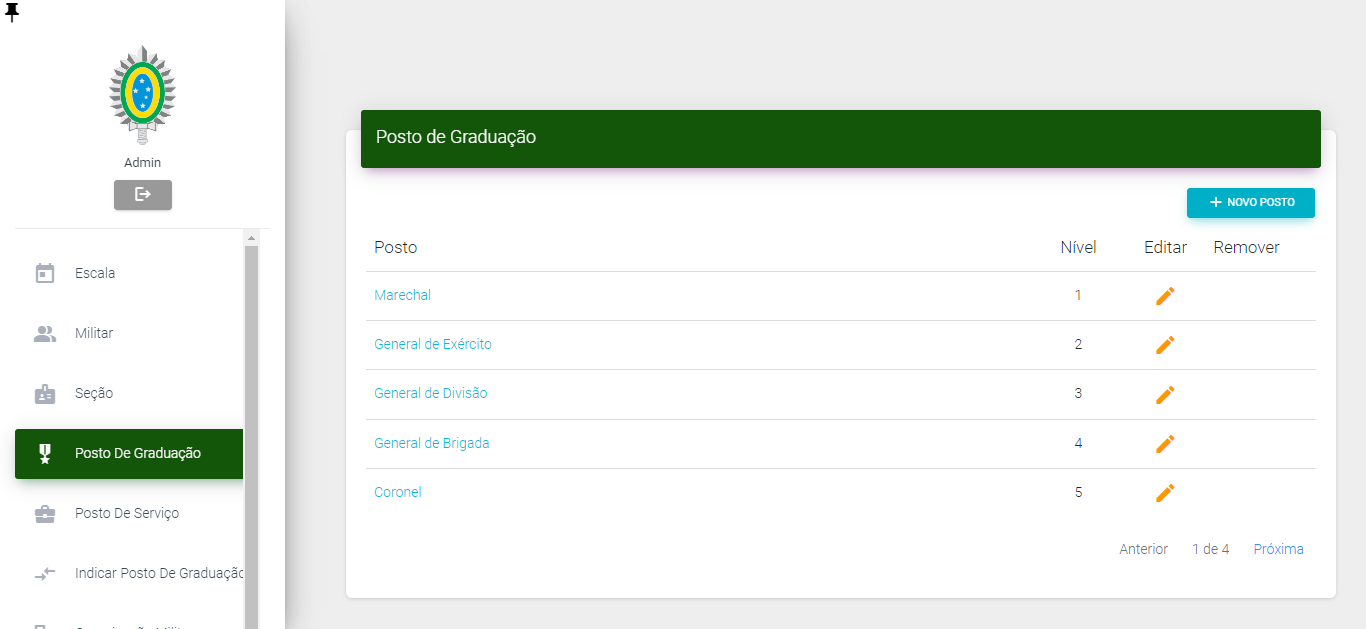
\includegraphics[width=0.8\textwidth]{images/10 - Posto de Graduacao.png}
    \label{fig:postograuacao}
\end{figure}


\subsection{Posto de Serviço}

O módulo de posto de serviço tem todas as funcionalidades necessárias para a manutenção dos postos de serviço. Os postos de serviços geridos por esse módulo, são os serviços para os quais os militares são escalados. A tela principal do módulo é apresentada na Figura \ref{fig:postoservico}, sendo as funcionalides de inserção e alteração disponíveis apenas para o usuario adminstrador.

\begin{figure}[!htb]
    \centering
    \caption{Posto de Serviço}
    \includegraphics[width=0.8\textwidth]{images/8 - Posto de Serviço.png}
    \label{fig:postoservico}
\end{figure}

Uma regra importante definida por esse módulo, é apontar qual a graduação necessária para cada posto de serviço, um militar que não tenha a graduação necessária definida nesse módulo é imcapaz de ser escalado para o serviço, um exemplo das graduações definidas para o posto é apresentada na Figura \ref{fig:viewpostoservico}.

\begin{figure}[!htb]
    \centering
    \caption{Visualizar Posto de Serviço }
    \includegraphics[width=0.8\textwidth]{images/8 - Posto de Serviço - Graduacao.png}
    \label{fig:viewpostoservico}
\end{figure}

\subsection{Indicar Gradução}

Esse módulo é responsável por atribuir graduações a um determinado posto de serviço, a graduação só poder ser vinculada uma unica vez para cada posto de serviço, evitando uplicidade. A Figura \ref{fig:indicargraducao}, apresenta o formulário de vinculação.

\begin{figure}[H]
    \centering
    \caption{Indicar Posto de Graduação}
    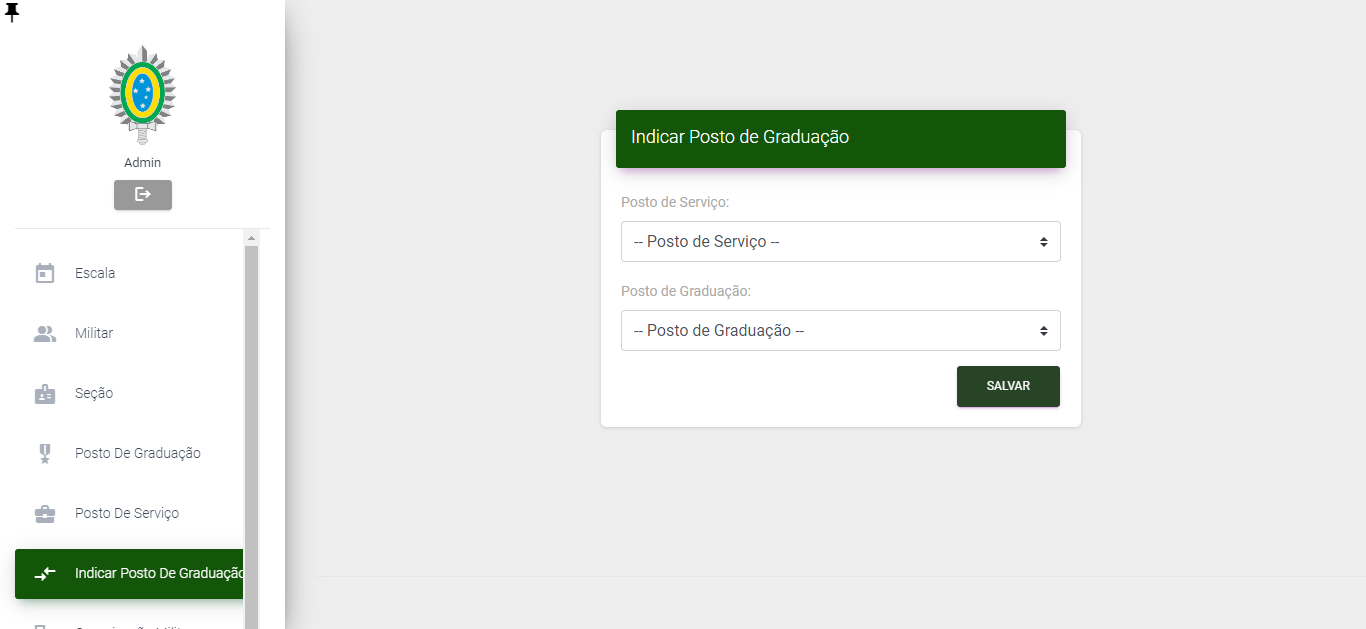
\includegraphics[width=0.8\textwidth]{images/9 - Indicar Graduação.png}
    \label{fig:indicargraducao}
\end{figure}

\subsection{Impedimento}

O módulo de impedimento define um período em que o militar não poderá ser escalado mediante à uma justificativa. Cada impedimento, tem uma data de início e fim determinado, e um documento comprobatório. Ná Figura \ref{fig:impedimento} é aprensentado o formulário de cadastro do impedimento de um militar.

\begin{figure}[H]
    \centering
    \caption{Cadastro de Impedimento}
    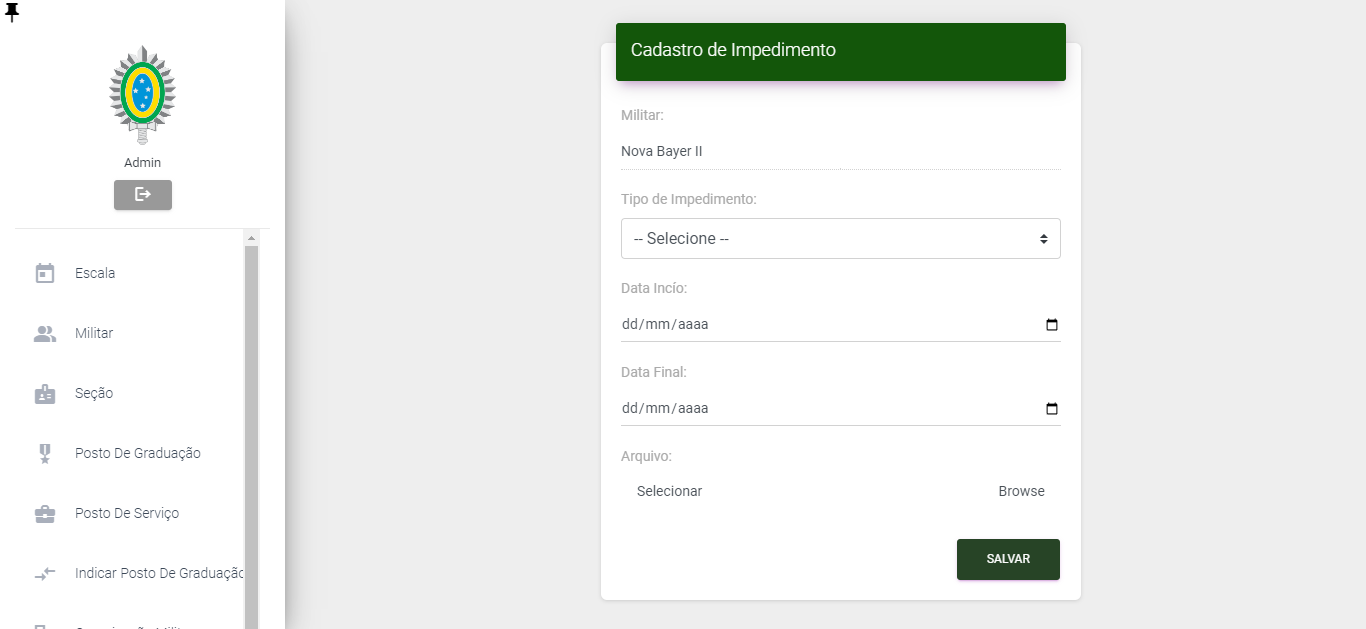
\includegraphics[width=0.8\textwidth]{images/11 - Impedimento.png}
    \label{fig:impedimento}
\end{figure}

\subsection{Auditoria}

A auditoria é feita salvado o registro de toda e qualquer alteração na base de dados. Qualquer discrepência ou irregularidade deve ser solicitada a verificação das alteração por meio de relatórios extraídos diretos da base de dados. A Figura \ref{fig:auditoria}, apresenta uma visualização dos dados de auditoria contidos na base para fins de exemplo, não sendo um módulo disponível no sistema.

\begin{figure}[H]
    \centering
    \caption{Registro de Auditoria}
    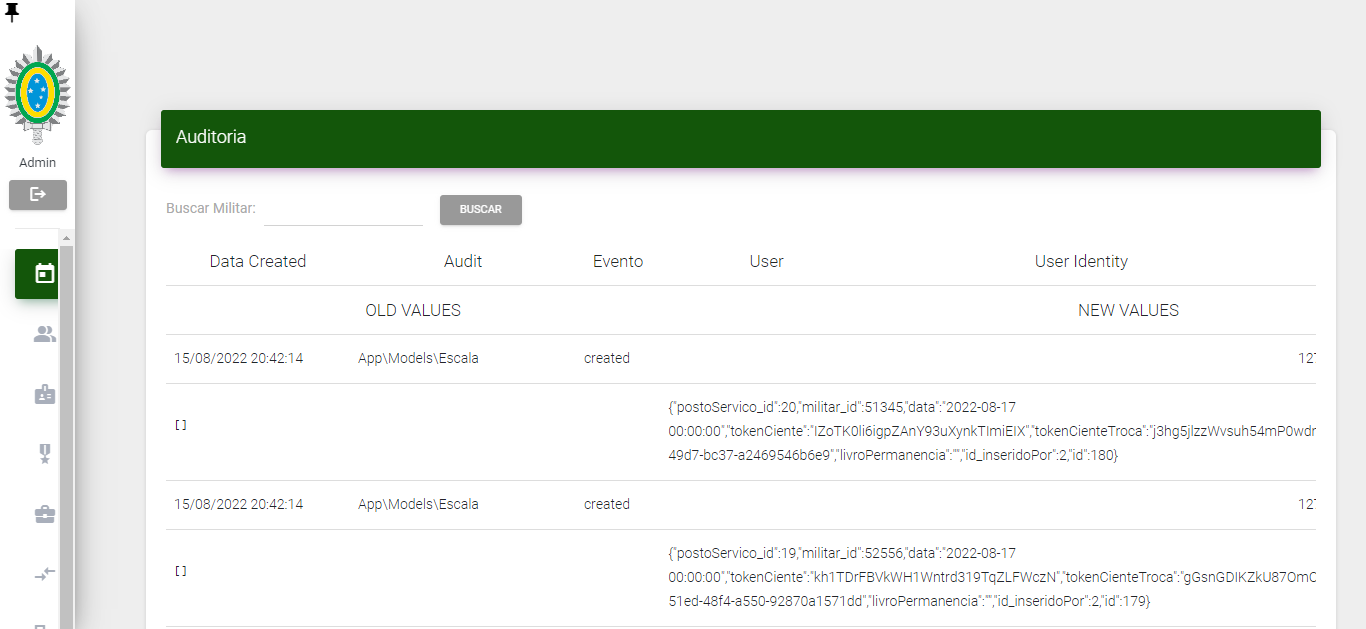
\includegraphics[width=0.8\textwidth]{images/TELA DE AUTIDORIA.png}
    \label{fig:auditoria}
\end{figure}
